%\documentclass[12pt,a4paper]{report}
\documentclass[12pt,a4paper,oneside,onecolumn,openright]{book}
% set the document language
\usepackage[italian]{babel}
% set the encoding used by your editor here (default is utf8)
\usepackage[utf8]{inputenc}

% math packages
\usepackage{amsmath}
\usepackage{amssymb}
% page margins settings
\usepackage[inner=3cm,outer=2.5cm,top=3cm,bottom=2.5cm]{geometry}
%\usepackage{indentfirst}


% other packages
\usepackage{array}
\usepackage{subfigure}
\usepackage{graphicx}
\usepackage{verbatim}
\usepackage{listings}
\usepackage{url}
\usepackage[hidelinks]{hyperref}
\usepackage{wrapfig,lipsum,booktabs}
% custom colors
\usepackage{xcolor}
\definecolor{light-gray}{gray}{0.96}
\definecolor{cyan}{RGB}{230,230,255}
\definecolor{dkgreen}{rgb}{0,0.6,0}
\definecolor{gray}{rgb}{0.5,0.5,0.5}
\definecolor{mauve}{rgb}{0.58,0,0.82}

\setcounter{section}{0}

\begin{document}
\begin{titlepage}
\begin{center}
{
    \large
    \textbf{Università  degli studi di Modena e Reggio Emilia} \\
   	\textbf{Dipartimento di Scienze Fisiche, Informatiche e Matematiche} \\
    \vspace{\stretch{0.5}}
    \hspace*{0cm} \hrulefill \hspace*{0cm} \\
    \vspace{\stretch{0.5}}
   	\emph{Corso di Laurea in Informatica}
    
	  \vspace{\stretch{12}}
  
  
 		\huge{\bf Strategie Innovative di Sicurezza}}\\
		\vspace{3mm}
		{\huge{\bf Informatica: monitoraggio delle reti}}\\
		\vspace{3mm}
		\vspace{3mm}
		{\huge{\bf  grazie a Darktrace e Tpot}}\\
		\vspace{3mm}
		\vspace{3mm}
		
		\vspace{\stretch{6}}
		\end{center}
		
\vspace{40mm}
\par
\noindent
\begin{minipage}[t]{0.47\textwidth}
{\large{\bf Relatore:\\
Prof.
Ferretti Luca}}\\ 
\\
\end{minipage}
\hfill
\begin{minipage}[t]{0.47\textwidth}\raggedleft
{\large{\bf Candidato:\\
Matteo Violi}}
\end{minipage}
\vspace{20mm}
\begin{center}
%\rule[0.1cm]{15.8cm}{0.1mm}
\hspace*{0cm} \hrulefill \hspace*{0cm} \\
{\large{\bf 
Anno Accademico 2023/2024}}
\end{center}

\end{titlepage}

\tableofcontents

\chapter{Introduzione}
\section{Contestualizzazione del tirocinio curricolare universitario}
\section{Scopo delle tesi}


\chapter{Fondamenti teorici su Honeypot e IDS}
\section{Introduzione agli honeypot}
\subsection{Definizione e scopo}
Nel 1989, Clifford Stoll pubblica quello che poi diventerà uno dei classici della 
letteratura sulla sicurezza informatica: \textbf{The Cuckoo's Egg}. 
Nel romanzo, Stoll racconta di aver scoperto un tentativo di intrusione informatica 
nei sistemi del laboratorio del Lawrence Berkeley National Laboratory, 
dove lavorava come astrofisico.\\
Analizzando delle discrepanze sulle fatture di addebito per l'uso di risorse informatiche 
e cercando di capirne la causa, Stoll inizia a seguire le tracce digitali lasciate, 
le quali lo condurranno fino a un hacker. Quest'ultimo si rivelò essere Markuss Hess, 
hacker tedesco famoso per aver violato sistemi più di quattrocento sistemi dell'esercito 
americano per poi vendere tutte le informazioni ai servizi di intelligence sovietici.\\
Hess venne scoperto grazie a un'idea di Stoll: un finto portale vulnerabile del 
Lawrence Berkeley National Laboratory. Questo gli permise di stabilire una connessione 
e localizzare il criminale. Stoll definì questa sua creazione una \textit{hoax}, 
una sorta di burla o truffa.\\
Uno dei primi documenti che trattava l'uso di trappole per attirare hacker malevoli 
fu redatto da William Cheswick, un pioniere della sicurezza informatica e l'ideatore di 
uno dei primi firewall. Cheswick creò quello che in quell'epoca chiamò \textit{roach motel}, 
una trappola progettata per intrappolare gli hacker, ispirandosi alla metafora di un 
motel per scarafaggi.\\
Nel corso degli anni, il termine \textit{honeypot} ha guadagnato sempre più popolarità, 
in quanto associato alla tradizione folkloristica dei popoli germanici, 
slavi e celtici. Secondo questa tradizione, gli orsi tendono a rubare il miele dagli 
alveari, un parallelismo che riflette l'idea di attirare e intrappolare gli 'hacker' 
simili a predatori.\\
In generale, un honeypot è costituito da un sistema informatico che simula un 
sistema legittimo, rendendolo vulnerabile ai più comuni attacchi informatici. 
L'obiettivo è di deviare l'attaccante dalle macchine reali e critiche, consentendo 
nel contempo lo studio dei loro comportamenti e delle tecniche di attacco durante e 
dopo la fase di \textit{exploitation}.\\

\subsection{Tipologie di honeypot}
Dal momento della loro concezione, possiamo categorizzare le diverse tipologie di 
honeypot in base alle risorse allocate o al contesto di utilizzo.\\
Per quanto riguarda le risorse, possiamo suddividerli in due categorie principali:
\begin{itemize}
	\item \textbf{Honeypot Fisici}: Questi utilizzano macchine reali con indirizzi IP 
	dedicati, simulando comportamenti modellati dal sistema. Tuttavia, questo modello 
	è raramente adottato a causa dell'alto costo di acquisizione, manutenzione e 
	delle specifiche esigenze hardware.
	\item \textbf{Honeypot Virtuali}: Questa tipologia consente l'installazione e la 
	simulazione di un host sulla rete, assegnando un indirizzo IP alla macchina virtuale. 
	Questo approccio è il più diffuso, offrendo un equilibrio tra efficacia e praticità.
\end{itemize}
Per quanto riguarda il contesto di utilizzo, possiamo distinguere:
\begin{itemize}
	\item \textbf{Honeypot di Produzione}: Questi honeypot sono progettati per un 
	utilizzo semplice, immagazzinano un numero limitato di informazioni e sono 
	spesso implementati in contesti aziendali. Collocati all'interno della rete 
	aziendale insieme agli altri server di produzione, raccolgono meno dati e 
	operano a bassa intensità.
	\item \textbf{Honeypot di Ricerca}: Questi honeypot sono finalizzati alla raccolta 
	di informazioni sulle metodologie di attacco degli aggressori. Non forniscono un 
	valore specifico a un'organizzazione particolare, ma sono più complessi da installare 
	e mantenere, raccogliendo un'ampia quantità di dati.
\end{itemize}
Recentemente, il mercato legato a questi servizi ha introdotto nuove tipologie 
di honeypot che estendono le funzionalità di base e incorporano tecniche di inganno, 
automatizzando la scalabilità su grandi reti. Le tipologie più diffuse includono:
\begin{itemize}
	\item \textbf{Honeypot malware}: Questi honeypot simulano un sistema vulnerabile 
	agli attacchi più comuni da parte di malware, consentendo uno studio approfondito 
	del malware, delle sue origini e del suo comportamento.
	\item \textbf{Honeypot spam}: Questi honeypot simulano relay di posta aperti o 
	proxy aperti, comunemente utilizzati dagli spammer. Ciò consente di rivelare 
	l'indirizzo IP dello spammer e fornire una cattura in blocco dello spam.
	\item \textbf{Honeypot database}: Questi honeypot simulano database con 
	possibili vulnerabilità, come ad esempio SQL Injection.
	\item \textbf{Honeypot ICS}: Questi honeypot simulano sistemi di controllo industriale 
	come i PLC (controller logico programmabile).
\end{itemize}
\newpage

\subsection{Tpot: panoramica}
La piattaforma T-Pot, sviluppata da Deutsche Telekom Security GmbH, è distribuita 
sotto licenza GPL-3.0, un modello copyleft per il software libero. 
Basata su Debian 11 per architetture amd64 e arm64, utilizza Docker e Docker-compose 
per eseguire simultaneamente una vasta gamma di strumenti e sfruttare appieno le 
risorse hardware dell'host. \\
T-Pot offre una serie di servizi suddivisi in cinque categorie principali:
\begin{enumerate}
	\item Connessione tramite SSH e Cockpit per la gestione attraverso un'interfaccia web. 
	\item Elastic Stack, composto da Elasticsearch per l'archiviazione dei dati, Logstash per l'analisi e Kibana per la visualizzazione su dashboard.
	\item Strumenti quali Cyberchef per la codifica e decodifica dei dati, Elasticvue per l'interazione con un cluster Elasticsearch, T-Pot Attack Map per la visualizzazione degli attacchi in tempo reale e Spiderfoot per l'automazione dell'OSINT.
	\item Honeypots, che includono una selezione di ventidue honeypot configurabili.
	\item Monitoraggio della rete attraverso Suricata, un motore di sicurezza di rete.
\end{enumerate}

\subsection{Tpot: scopo e utilità in ambiente di tirocinio}
Nell'ambito del tirocinio, lo scopo e l'utilità di T-Pot è stato quello di testare e 
configurare la piattaforma al fine di generare e inviare avvisi a Sentinel, il sistema 
SIEM aziendale. L'obiettivo principale era quello di condurre prove in un ambiente 
controllato prima di implementare la soluzione su un server in produzione. 
Inoltre, si è pianificato di redigere un manuale dettagliato che documentasse tutti i 
passaggi per l'installazione e la configurazione di T-Pot, rendendolo accessibile anche 
a utenti non esperti. Questo avrebbe consentito una rapida e agevole adozione della 
soluzione da parte dell'azienda e avrebbe fornito una guida utile per futuri aggiornamenti e manutenzioni.
\newpage

\section{Teoria sugli IDS}
\subsection{Evoluzione e storia degli IDS}
\begin{wraptable}{r}{0.45\textwidth}
	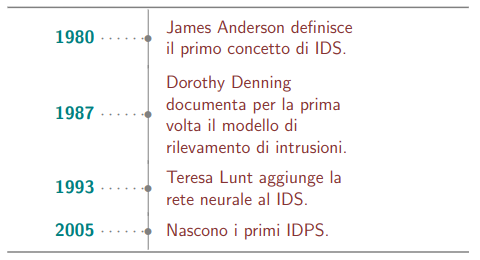
\includegraphics[width=0.45\textwidth]{IDStimeline.png}
\end{wraptable} 
Il primo concetto preliminare di sistema di rilevamento delle intrusioni (IDS) 
è stato descritto nel 1980 da James Anderson presso la National Security Agency 
e comprendeva un insieme di strumenti per gli amministratori per esaminare i registri 
di audit. Nel febbraio del 1987, Dorothy E. Denning, assistita da Peter G. Neumann 
presso IDS International, pubblicò un documento intitolato "An Intrusion Detection Model".\\
Questo modello presentava un sistema esperto basato su regole per rilevare pattern 
di intrusioni note e una componente di rilevazione statistica basata su profili di 
utenti, sistemi host e sistemi di destinazione, diventando noto come Intrusion Detection 
Expert System.\\
Nel 1993, Teresa F. Lunt, autrice di "IDES: An Intelligent System for Detecting Intruders", 
aggiunse l'ultimo componente al modello di Denning: una rete neurale artificiale capace di 
adattarsi agli eventi e modificarsi. \\
Un sistema di rilevamento delle intrusioni (IDS) è un dispositivo software o un'applicativo 
che monitora una rete o i dispositivi su cui è installato. Quando rileva un'anomalia, 
la segnala a un sistema di raccolta di eventi di sicurezza (SIEM), che utilizza tecniche 
di filtraggio degli allarmi per distinguere falsi positivi da attività dannose.\\
Gli IDS, come un firewall, vengono utilizzati per prevenire intrusioni nella rete, 
ma differiscono dalla risposta a tali intrusioni. I sistemi di rilevamento delle 
intrusioni possono anche avere scopi specifici integrandoli con strumenti personalizzati, 
come l'utilizzo di un honeypot per attirare e caratterizzare il traffico dannoso.\\
Recentemente, alcuni prodotti IDS hanno la capacità di rispondere alle intrusioni 
rilevate, denominati sistemi di rilevamento e prevenzione delle intrusioni (IDPS). 
Gli IDPS aggiungono la capacità di fermare un attacco rilevato, registrare gli eventi, 
avvisare gli amministratori, bloccare la minaccia e generare rapporti. A differenza 
degli IDS, gli IDPS devono essere posizionati "in linea", monitorando in tempo reale 
per bloccare intrusioni, inviare allarmi, rifiutare pacchetti dannosi e correggere 
errori di rete.\\


\subsection{Tipologie di IDS}
La classificazione tipica dei sistemi di intrusione si basa sulla loro posizione:
\begin{itemize}
	\item \textbf{NIDS (Network IDS)}: Posizionati strategicamente nella rete, 
	monitorano il traffico da e verso tutti i dispositivi, analizzando idealmente 
	sia l'entrata che l'uscita. L'uso di reti neurali artificiali può migliorare i 
	tassi di rilevamento grazie alla capacità di analizzare grandi volumi di dati 
	in modo intelligente e apprendere dagli errori, sviluppando un sistema di avviso precoce.
	\item \textbf{HIDS (Host IDS)}: Operano su singoli host o dispositivi, monitorando 
	solo i pacchetti in entrata e in uscita. Consentono l'analisi del traffico di rete 
	criptato, una volta arrivato all'host.
\end{itemize}
Gli IDS possono essere classificati anche in base all'approccio di rilevamento:
\begin{itemize}
	\item \textbf{Signature-based}: Ricerca pattern specifici, simile all'azione degli 
	antivirus per individuare sequenze di byte o istruzioni malevole conosciute. 
	Risponde velocemente a attacchi noti, ma può non riconoscere nuovi attacchi senza pattern noti.
	\item \textbf{Anomaly-based}: Utilizza l'apprendimento automatico per creare un 
	modello di attività affidabile e confrontare il nuovo comportamento. Riesce a 
	rilevare attacchi sconosciuti, ma potrebbe generare falsi positivi, identificando 
	attività legittime come malevoli.
\end{itemize}

\subsection{Darktrace: panoramica}
Darktrace, fondata nel 2013 a Cambridge, Regno Unito, da ex-dipendenti dell'intelligence 
governativa e matematici dell'Università di Cambridge, è un Intrusion Detection and 
Prevention System (IDPS) che immagazzina e analizza il traffico di rete per lunghi 
periodi al fine di identificare correlazioni e modelli comportamentali.\\

Utilizzando avanzate tecniche di probabilità bayesiana e machine learning, Darktrace 
crea un profilo comportamentale unico per ciascun utente e dispositivo all'interno 
dell'ambiente di rete. Inoltre, è in grado di raggruppare gli utenti e i dispositivi 
in base ai loro comportamenti, consentendo così di rilevare anomalie nel caso in cui 
un utente o un dispositivo si discosti dal comportamento tipico del suo gruppo.\\

Operando in tempo reale e analizzando il traffico di rete in modo continuo, Darktrace 
è in grado di identificare anche gli attacchi "zero-day", che non seguono schemi precedentemente 
noti. Per garantire l'affidabilità delle segnalazioni, Darktrace utilizza un'intelligente 
soglia di rilevamento che contestualizza e aggiorna costantemente le segnalazioni in 
base alle rilevazioni precedenti, riducendo al minimo i falsi positivi e mitigando il 
rischio di distorsioni dovute al tasso di base.\\

Darktrace è composto da quattro moduli distinti: Darktrace PREVENT, Darktrace DETECT, 
Darktrace RESPOND e Darktrace HEAL. Tuttavia, durante il tirocinio, ci concentreremo 
esclusivamente sui moduli DETECT e RESPOND, in quanto sono gli unici utilizzati durante 
l'esperienza pratica.

\subsection{Darktrace DETECT}
\subsection{Darktrace RESPOND}
Darktrace RESPOND/Network è progettato per gestire minacce di sicurezza di alto livello, 
come ad esempio i ransomware. Utilizzando due approcci distinti, può interrompere le 
connessioni malevole sia attraverso il reset TCP che integrandosi direttamente con 
il firewall esistente, inviando messaggi direttamente a esso.\\

Il flag RST del protocollo TCP è una componente delle comunicazioni standard tra 
dispositivi: quando un endpoint riceve un pacchetto con questo flag attivato, 
la connessione viene immediatamente interrotta. Darktrace rileva attività sospette e, 
in caso di anomalie, invia pacchetti di reset TCP a entrambi i dispositivi coinvolti, 
sia all'interno che all'esterno della rete, per interrompere la connessione malevola. 
Gli indirizzi IP dei pacchetti di reset sono falsificati per far credere ai dispositivi 
che non provengano da Darktrace, ma l'uno dall'altro.\\

Darktrace RESPOND può attuare una serie di azioni proattive, misurate e automatizzate 
in risposta a minacce informatiche confermate rilevate in tempo reale.\\

I componenti di Darktrace RESPOND possono essere utilizzati in due modalità distinte:
\begin{itemize}
	\item \textbf{Modalità di conferma umana}: le azioni di Darktrace RESPOND rimarranno in 
	sospeso fino a quando un operatore umano non conferma o ignora 
	la segnalazione del modulo RESPOND.
	\item \textbf{Modalità autonoma o parzialmente autonoma}: in modalità completamente 
	autonoma, RESPOND risponde automaticamente alle minacce, mentre nella modalità 
	parzialmente autonoma, può essere attivato autonomamente al di fuori degli orari 
	lavorativi, ma richiede conferma umana per il resto del tempo.
\end{itemize}


Darktrace RESPOND reagisce alle violazioni dei modelli offrendo l'opzione di impostare 
un inibitore, che è un'azione finalizzata a contrastare il comportamento anomalo del 
dispositivo o dell'utente. Gli inibitori disponibili includono:
\begin{itemize}
	\item \textbf{Bloccare le connessioni corrispondenti}: Questa opzione interrompe le 
	connessioni dal dispositivo all'endpoint di destinazione identificato nell'incidente, 
	sulla porta di destinazione osservata.
	\item \textbf{Imporre il pattern di vita}: Questa funzione consente al dispositivo 
	di effettuare solo connessioni e trasferimenti di dati considerati normali da 
	Darktrace, basati sui modelli di vita definiti per quel dispositivo. 
	Qualsiasi attività che si discosti da questi modelli viene bloccata.
	\item \textbf{Imporre il pattern di vita del gruppo}: Questa opzione permette al 
	dispositivo di intraprendere le stesse connessioni e trasferimenti di dati che 
	sono comuni tra i dispositivi nel suo gruppo di pari, basandosi sui modelli di vita 
	del gruppo.
	\item \textbf{Quarantena del dispositivo}: Questa azione blocca tutto il traffico di 
	rete in entrata e in uscita dal dispositivo, isolandolo dalla rete.
	\item \textbf{Blocco di tutti i traffici in uscita}.
	\item \textbf{Blocco di tutti i traffici in entrata}.
\end{itemize}

\chapter{Sperimentazione con Tpot e Darktrace}
\section{Implementazione di Tpot e analisi dei risultati}
\subsection{Configurazione di base}
\subsection{Simulazione di server in produzione}
\subsection{Dati raccolti}
\subsection{Esperienze pratiche durante il tirocinio}

\section{Monitoraggio delle reti con Darktrace}
\subsection{Studi di caso}
\subsection{Esempi di minacce rilevate}

\section{Integrare Darktrace e Tpot per una maggiore sicurezza}

\chapter{Conclusioni}
\section{Riassunto delle principali conclusioni}
\section{Riflessioni personali sull'esperienza di tirocinio}
\section{Suggerimenti per future ricerche o sviluppi in questo ambito}

\chapter{Bibliografia}

\chapter{Ringraziamenti}

\end{document}
